\documentclass[10pt]{article}
\usepackage{graphicx}
\usepackage{array}
\usepackage{booktabs}
\usepackage[margin=3cm, top=5cm, headheight=90pt]{geometry}
\usepackage{cmbright}
\usepackage[OT1]{fontenc}
\usepackage{float}
\usepackage[table]{xcolor}
\usepackage{pgfplots}
\pgfplotsset{compat=newest}
\usepackage{caption}
\usepackage{subcaption}
\usepackage{fancyhdr}
\usepackage{blindtext}
\usepackage{wrapfig}
\usepackage{amsmath}
\usepackage{natbib}
\setcitestyle{square}
\usepackage{url}
\usepackage{longtable}
\usepackage{parskip}

\pagestyle{fancy}
\rhead{\includegraphics[width=0.2\textwidth]{/Users/finn/Documents/Cardiff-University-logo-for-website}}
\lhead{{\large PX2155 Observational Techniques in Astronomy \\ Electronic Laboratory Diary} \\ Determining the ages of stellar clusters \\ \today \\ Finnbar Wilson \vspace{0.6cm}}

\begin{document}
\section{Aims and Objectives}
In this report images of the globular cluster M13 taken by the 3.6m Canada-France-Hawaii Telescope (CFHT) on the 16th of February 2001 will be used to analyse the composition of M13 and therefore predict its age. The data obtained will then be compared to publicly available results and experiments to discuss the accuracy of this experiment.
\section{Plan}
In this experiment, the subsequent outline will be followed in order to ensure that the report meets all of the scientific goals as listed below:
\begin{itemize}
	\item Import the fits files of the cluster M13 in the V and B filters into Gaia.
	\item Find several stars of known magnitude and compare to the aperture photometry results obtained in Gaia so that the zero point magnitude can be obtained.
	\item Record the magnitudes of at least 80 stars taking into consideration the zero point magnitude
	\item Create a Hertzsprung-Russell (H-R) diagram and compare it to an isochrone model to find the main sequence turn off point and therefore the age of the cluster
	\item Using publicly available data of M13 plot another H-R diagram and compare the results with those obtained in this report.
\end{itemize}
\section{Risk Assessment}
This experiment has little to no risk so it is safe to carry out the experiment.
\begin{table}[H]
	\centering
	\caption{Risk Assessment}
	\begin{tabular}{p{0.2\textwidth}p{0.65\textwidth}}
		\toprule
		Risk & Mitigation \\
		\midrule
		Tripping & Place trip hazards under desk \\
		\addlinespace
		\cellcolor{gray!10} Electric shock & \cellcolor{gray!10} Do not drink water in the lab \\
		\addlinespace
		Sitting for long period of time & Can cause wrist and band injuries so take frequent breaks to stand up and stretch. \\
		\bottomrule
	\end{tabular}
\end{table}
\pagebreak
\section{Context: Techniques to determine the age of stellar clusters}

\begin{wrapfigure}{r}{0.47\textwidth}
	\vspace{-1.1\intextsep}
	\centering
	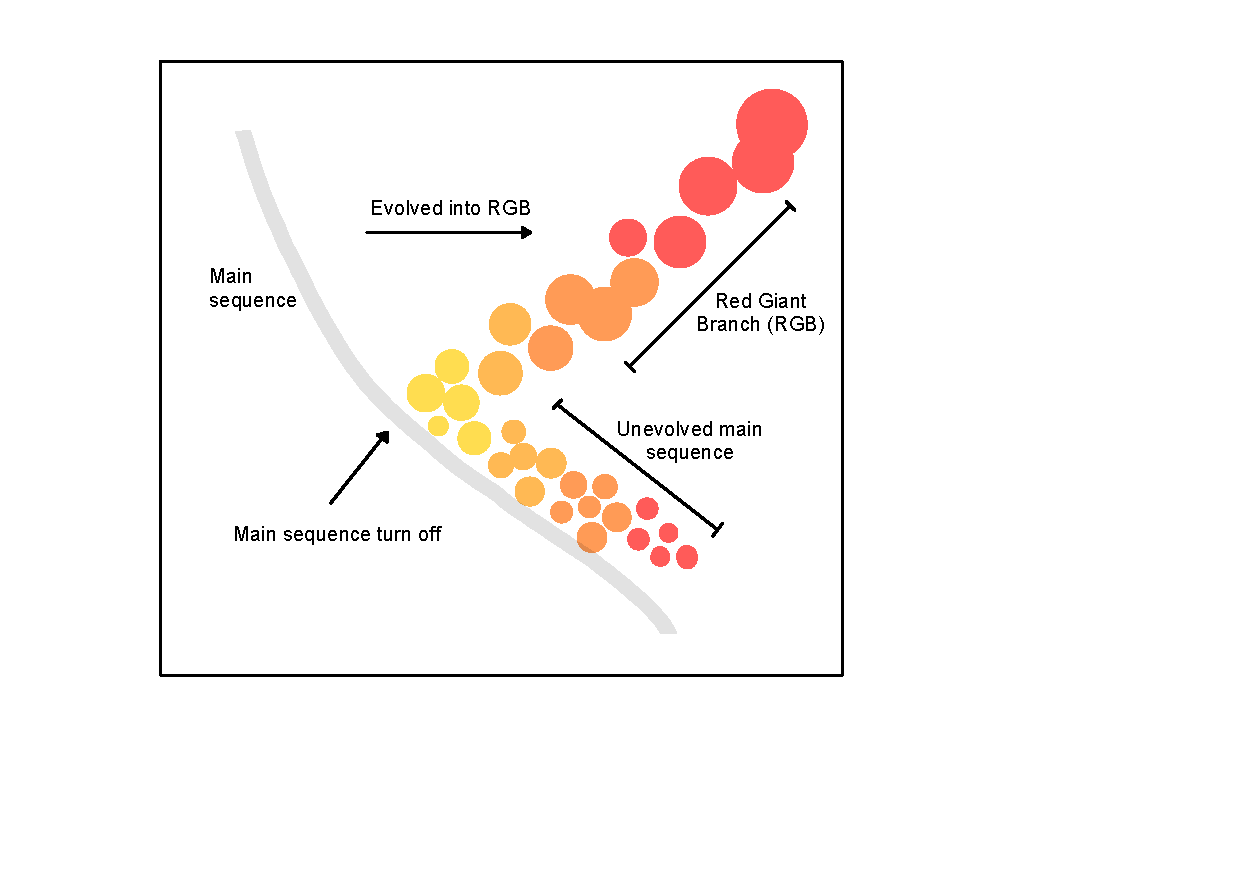
\includegraphics[width=0.47\textwidth]{Cluster}
	\caption{H-R diagram showing the main sequence turn off for clusters}
	\label{fig:mainseq}
\end{wrapfigure}

The main technique utilised to find the age of stellar cluster is comparing the Hertzsprung-Russell diagram of the cluster to theoretical models of the stellar contents called isochrones and inferring the age based on the similarities. One of the identifiers to the age of the cluster is the main sequence turn off; this is where more luminous stars on the main sequence  evolve into the red giant branch (RGB). As stellar evolutions are well studied information on what age stars evolve onto the RGB can be easily found. This then means that the age of the cluster is equal to the age where a star on the main sequence turn off would evolve \citep{lick}. Isochrone models work for every cluster with a similar composition as the arrangement of stars does not play a vital role the evolution of the cluster. Another way of determining cluster age is by observing the cluster dynamics as the interactions of stars within the cluster can give insights into its age. 

\section{Methods}

To obtain accurate measurements of the magnitudes of stars in M13 Gaia needs to be calibrated. 7 stars were chosen as calibration references with known magnitudes in the V and B filter and are listed by A to G in Figure \ref{fig:position}. Once the magnitude of the star in Gaia is known (instrument magnitude, $m_{\text{instr}}$) then it can be compared with the actual magnitude, $m_{\text{star}}$, to find the difference in magnitude called the zero point magnitude, $m_{\text{zp}}$, as shown by Equation \ref{eq:cal}.
\begin{equation}
	m_{\text{star}} = m_{\text{zp}} + m_{\text{instr}}
	\label{eq:cal}
\end{equation}
This then means that any further aperture photometry done in Gaia can be calibrated to account for this difference in magnitude. This process has to be done in both the V and B filter as they have different zero point magnitudes.

\begin{wrapfigure}{R}{0.29\textwidth}
	\centering
	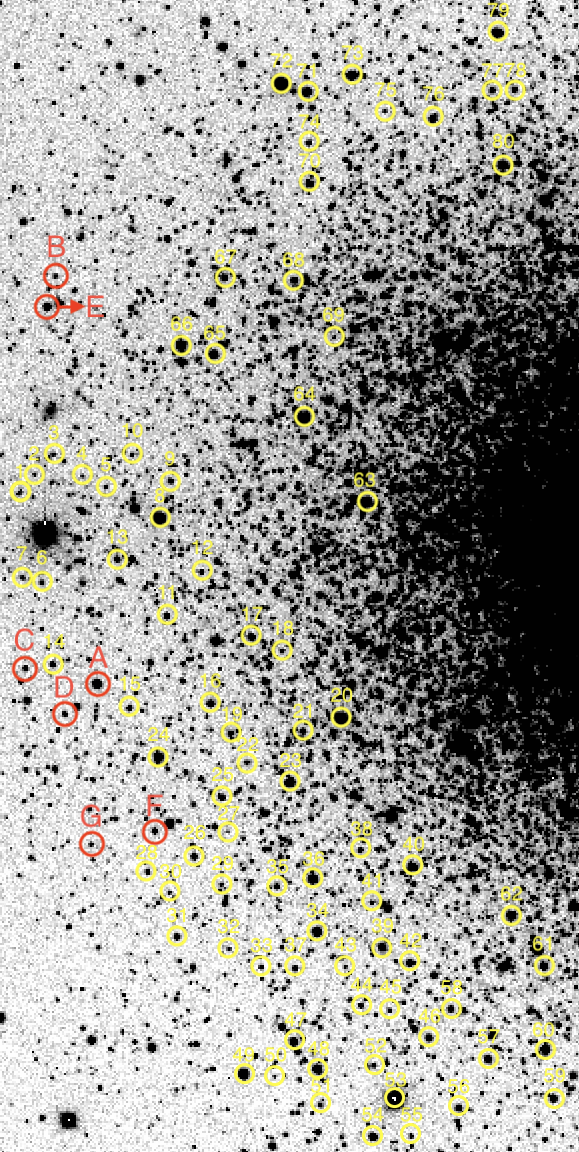
\includegraphics[width=0.29\textwidth]{positions}
	\caption{Position of the stars used to calibrate the zero point magnitude of the FITs image}
	\label{fig:position}
\end{wrapfigure}

The actual apparent magnitudes of the stars in the V band are listed by V$_{\text{star}}$ in Table \ref{tab:Vzp} with their associated error from the \citet{labhandbook}. The image of M13 in the V filter was then opened in Gaia and the stars A to G were identified. Using the aperture photometry tool the magnitude of each star was recorded along with their uncertainty and is shown as V$_{ \text{instr}}$ in Table \ref{tab:Vzp}. Equation \ref{eq:cal} was then used to find the zero point magnitude of each star. The average zero point magnitude in the V filter was $-18.885 \pm 0.004$. The actual apparent magnitudes of the stars in the B band are listed by B$_{ \text{star}}$ in Table \ref{tab:Bzp} with their associated error from the \citet{labhandbook}. The same method to find the zero point magnitude in the V filter was used in finding the zero point magnitude in the B filter which obtained an average value of $-18.329 \pm 0.004$

As the initial frame point magnitude in Gaia was set as 50 for both V and B magnitudes, to calibrate the aperture photometry tool to display the correct magnitudes the zero point magnitude need to be added to 50. This was then tested to determine if the calibration was successful on each of the stars listed in Table \ref{tab:zp}. This test produced roughly the same magnitudes as those in Table \ref{tab:zp} so the calibration of Gaia was successful. Using the aperture photometry tool a circular aperture was created around each of the stars shown by the yellow circles in Figure \ref{fig:position} as well as recording their positions to ensure that the correct stars were selected in both the V and B filter. only the star was enclosed in the circular aperture so the radius of aperture was slightly larger than the radius of the star. I repeated this process for all 80 stars. The results are shown by the apparent magnitude column of Table \ref{tab:table}. To create a H-R diagram of M13 the magnitudes need to be converted from apparent to absolute. This can be done using Equation \ref{eq:mag}.
\begin{equation}
	M = m - 5 \log _{10}\left(\frac{d}{10}\right)
	\label{eq:mag}
\end{equation}
Where $M$ is absolute magnitude, $m$ is apparent magnitude and $d$ is the distance to the star is parsecs. The distance to each of the stars was approximated as the distance to M13 which is 6.8 kpc \citep[Table 4]{Paust_2010}. The absolute magnitude of each star is shown in the absolute column of Table \ref{tab:table}. The errors in the values in Table \ref{tab:table} are from the error in recording the magnitudes using the aperture photometry tool which is calculated by Gaia. A larger version of Figure \ref{fig:position} is in the appendix.
\begin{table}[H]
	\caption{Calibration stars apparent magnitudes in both V and B filters}
	\begin{subtable}{.5\linewidth}
	\centering
	\caption{V Magnitudes of standard stars}
	\begin{tabular}{c|cc|cc}
		Star & V$_{ \text{star}}$ & V$_{ \text{star err}}$ & V$_{ \text{instr}}$ & V$_{ \text{instr err}}$ \\
		\midrule
		A &  14.952 &  0.007 &  33.836 &  0.001 \\
		B &  18.304 &  0.008 &  37.184 &  0.008 \\
		C &  17.510 &  0.007 &  36.412 &  0.004 \\
		D &  17.914 &  0.007 &  36.768 &  0.007 \\
		E &  15.875 &  0.006 &  34.751 &  0.002 \\
		F &  16.925 &  0.007 &  35.814 &  0.003 \\
		G &  18.494 &  0.008 &  37.403 &  0.012 \\ 
	\end{tabular}
	\label{tab:Vzp}
	\end{subtable}
	\begin{subtable}{.5\linewidth}
	\caption{B Magnitudes of standard stars}
	\begin{tabular}{c|cc|cc}
		Star & B$_{ \text{star}}$ & B$_{ \text{star err}}$ & B$_{ \text{instr}}$ & B$_{ \text{instr err}}$ \\
		\midrule
		A &  15.745 &  0.010 &  34.077 &  0.001 \\
		B &  18.744 &  0.010 &  37.063 &  0.008 \\
		C &  18.157 &  0.011 &  36.491 &  0.005 \\
		D &  18.452 &  0.011 &  36.777 &  0.006 \\
		E &  15.817 &  0.010 &  34.121 &  0.001 \\
		F &  17.602 &  0.010 &  35.939 &  0.003 \\
		G &  18.928 &  0.010 &  37.279 &  0.009 \\ 
	\end{tabular}
	\label{tab:Bzp}
	\end{subtable}
	\caption*{Stars A to G positions are shown in Figure \ref{fig:position}. The errors associated with these values are calculated in the aperture photometry tool in Gaia.}
	\label{tab:zp}
\end{table}

\pagebreak

\begin{longtable}[c]{ccccc|cccc}
\caption{Magnitude of stars in M13 \label{tab:table}} \\

	& \multicolumn{4}{c}{Apparent} &  \multicolumn{4}{c}{Absolute} \\
	\cmidrule(lr){2-9}
	Star & V & V$_{ \text{err}}$ & B & B$_{ \text{err}}$ & V & V$_{ \text{err}}$ & B & B$_{ \text{err}}$ \\
	\midrule
	\endhead
		 
	\bottomrule
	\endfoot
		 
1 & \cellcolor{ gray!10 }  19.854 &  0.029 & \cellcolor{ gray!10 }  19.291 &  0.012 & \cellcolor{ gray!10 }  5.691 &  0.029 & \cellcolor{ gray!10 }  5.129 &  0.012 \\
2 & \cellcolor{ gray!10 }  19.338 &  0.018 & \cellcolor{ gray!10 }  19.793 &  0.017 & \cellcolor{ gray!10 }  5.175 &  0.018 & \cellcolor{ gray!10 }  5.630 &  0.017 \\
3 & \cellcolor{ gray!10 }  18.837 &  0.010 & \cellcolor{ gray!10 }  19.259 &  0.010 & \cellcolor{ gray!10 }  4.674 &  0.010 & \cellcolor{ gray!10 }  5.097 &  0.010 \\
4 & \cellcolor{ gray!10 }  19.956 &  0.026 & \cellcolor{ gray!10 }  20.534 &  0.029 & \cellcolor{ gray!10 }  5.793 &  0.026 & \cellcolor{ gray!10 }  6.372 &  0.029 \\
5 & \cellcolor{ gray!10 }  18.938 &  0.012 & \cellcolor{ gray!10 }  19.365 &  0.013 & \cellcolor{ gray!10 }  4.776 &  0.012 & \cellcolor{ gray!10 }  5.203 &  0.013 \\
6 & \cellcolor{ gray!10 }  17.812 &  0.006 & \cellcolor{ gray!10 }  18.383 &  0.006 & \cellcolor{ gray!10 }  3.649 &  0.006 & \cellcolor{ gray!10 }  4.220 &  0.006 \\
7 & \cellcolor{ gray!10 }  18.992 &  0.014 & \cellcolor{ gray!10 }  20.455 &  0.027 & \cellcolor{ gray!10 }  4.829 &  0.014 & \cellcolor{ gray!10 }  6.292 &  0.027 \\
8 & \cellcolor{ gray!10 }  13.518 &  0.000 & \cellcolor{ gray!10 }  14.364 &  0.000 & \cellcolor{ gray!10 } -0.645 &  0.000 & \cellcolor{ gray!10 }  0.201 &  0.000 \\
9 & \cellcolor{ gray!10 }  17.350 &  0.004 & \cellcolor{ gray!10 }  18.004 &  0.004 & \cellcolor{ gray!10 }  3.187 &  0.004 & \cellcolor{ gray!10 }  3.841 &  0.004 \\
10 & \cellcolor{ gray!10 }  18.870 &  0.011 & \cellcolor{ gray!10 }  19.323 &  0.012 & \cellcolor{ gray!10 }  4.708 &  0.011 & \cellcolor{ gray!10 }  5.161 &  0.012 \\
11 & \cellcolor{ gray!10 }  17.241 &  0.004 & \cellcolor{ gray!10 }  17.855 &  0.004 & \cellcolor{ gray!10 }  3.079 &  0.004 & \cellcolor{ gray!10 }  3.693 &  0.004 \\
12 & \cellcolor{ gray!10 }  17.820 &  0.005 & \cellcolor{ gray!10 }  18.366 &  0.007 & \cellcolor{ gray!10 }  3.657 &  0.005 & \cellcolor{ gray!10 }  4.203 &  0.007 \\
13 & \cellcolor{ gray!10 }  17.137 &  0.003 & \cellcolor{ gray!10 }  17.775 &  0.004 & \cellcolor{ gray!10 }  2.975 &  0.003 & \cellcolor{ gray!10 }  3.613 &  0.004 \\
14 & \cellcolor{ gray!10 }  17.073 &  0.003 & \cellcolor{ gray!10 }  17.740 &  0.003 & \cellcolor{ gray!10 }  2.911 &  0.003 & \cellcolor{ gray!10 }  3.578 &  0.003 \\
15 & \cellcolor{ gray!10 }  17.507 &  0.004 & \cellcolor{ gray!10 }  18.097 &  0.005 & \cellcolor{ gray!10 }  3.345 &  0.004 & \cellcolor{ gray!10 }  3.934 &  0.005 \\
16 & \cellcolor{ gray!10 }  15.914 &  0.002 & \cellcolor{ gray!10 }  16.633 &  0.002 & \cellcolor{ gray!10 }  1.751 &  0.002 & \cellcolor{ gray!10 }  2.470 &  0.002 \\
17 & \cellcolor{ gray!10 }  16.179 &  0.002 & \cellcolor{ gray!10 }  16.871 &  0.002 & \cellcolor{ gray!10 }  2.016 &  0.002 & \cellcolor{ gray!10 }  2.709 &  0.002 \\
18 & \cellcolor{ gray!10 }  18.809 &  0.013 & \cellcolor{ gray!10 }  19.252 &  0.011 & \cellcolor{ gray!10 }  4.647 &  0.013 & \cellcolor{ gray!10 }  5.090 &  0.011 \\
19 & \cellcolor{ gray!10 }  17.025 &  0.003 & \cellcolor{ gray!10 }  17.678 &  0.004 & \cellcolor{ gray!10 }  2.862 &  0.003 & \cellcolor{ gray!10 }  3.516 &  0.004 \\
20 & \cellcolor{ gray!10 }  13.722 &  0.000 & \cellcolor{ gray!10 }  14.543 &  0.001 & \cellcolor{ gray!10 } -0.441 &  0.000 & \cellcolor{ gray!10 }  0.381 &  0.001 \\
21 & \cellcolor{ gray!10 }  17.174 &  0.003 & \cellcolor{ gray!10 }  17.173 &  0.003 & \cellcolor{ gray!10 }  3.012 &  0.003 & \cellcolor{ gray!10 }  3.010 &  0.003 \\
22 & \cellcolor{ gray!10 }  18.304 &  0.008 & \cellcolor{ gray!10 }  18.759 &  0.007 & \cellcolor{ gray!10 }  4.141 &  0.008 & \cellcolor{ gray!10 }  4.597 &  0.007 \\
23 & \cellcolor{ gray!10 }  14.909 &  0.001 & \cellcolor{ gray!10 }  15.694 &  0.001 & \cellcolor{ gray!10 }  0.746 &  0.001 & \cellcolor{ gray!10 }  1.531 &  0.001 \\
24 & \cellcolor{ gray!10 }  14.485 &  0.001 & \cellcolor{ gray!10 }  15.329 &  0.001 & \cellcolor{ gray!10 }  0.323 &  0.001 & \cellcolor{ gray!10 }  1.167 &  0.001 \\
25 & \cellcolor{ gray!10 }  16.863 &  0.003 & \cellcolor{ gray!10 }  17.527 &  0.004 & \cellcolor{ gray!10 }  2.701 &  0.003 & \cellcolor{ gray!10 }  3.364 &  0.004 \\
26 & \cellcolor{ gray!10 }  17.049 &  0.003 & \cellcolor{ gray!10 }  17.703 &  0.004 & \cellcolor{ gray!10 }  2.886 &  0.003 & \cellcolor{ gray!10 }  3.541 &  0.004 \\
27 & \cellcolor{ gray!10 }  20.145 &  0.029 & \cellcolor{ gray!10 }  20.709 &  0.034 & \cellcolor{ gray!10 }  5.983 &  0.029 & \cellcolor{ gray!10 }  6.546 &  0.034 \\
28 & \cellcolor{ gray!10 }  17.623 &  0.005 & \cellcolor{ gray!10 }  18.335 &  0.007 & \cellcolor{ gray!10 }  3.461 &  0.005 & \cellcolor{ gray!10 }  4.173 &  0.007 \\
29 & \cellcolor{ gray!10 }  18.842 &  0.010 & \cellcolor{ gray!10 }  19.522 &  0.014 & \cellcolor{ gray!10 }  4.679 &  0.010 & \cellcolor{ gray!10 }  5.360 &  0.014 \\
30 & \cellcolor{ gray!10 }  18.919 &  0.012 & \cellcolor{ gray!10 }  19.319 &  0.012 & \cellcolor{ gray!10 }  4.756 &  0.012 & \cellcolor{ gray!10 }  5.156 &  0.012 \\
31 & \cellcolor{ gray!10 }  16.698 &  0.003 & \cellcolor{ gray!10 }  17.374 &  0.003 & \cellcolor{ gray!10 }  2.535 &  0.003 & \cellcolor{ gray!10 }  3.211 &  0.003 \\
32 & \cellcolor{ gray!10 }  18.861 &  0.011 & \cellcolor{ gray!10 }  19.364 &  0.010 & \cellcolor{ gray!10 }  4.699 &  0.011 & \cellcolor{ gray!10 }  5.201 &  0.010 \\
33 & \cellcolor{ gray!10 }  18.176 &  0.007 & \cellcolor{ gray!10 }  19.610 &  0.015 & \cellcolor{ gray!10 }  4.014 &  0.007 & \cellcolor{ gray!10 }  5.447 &  0.015 \\
34 & \cellcolor{ gray!10 }  15.052 &  0.001 & \cellcolor{ gray!10 }  15.141 &  0.001 & \cellcolor{ gray!10 }  0.889 &  0.001 & \cellcolor{ gray!10 }  0.978 &  0.001 \\
35 & \cellcolor{ gray!10 }  17.206 &  0.004 & \cellcolor{ gray!10 }  17.864 &  0.004 & \cellcolor{ gray!10 }  3.043 &  0.004 & \cellcolor{ gray!10 }  3.701 &  0.004 \\
36 & \cellcolor{ gray!10 }  14.589 &  0.001 & \cellcolor{ gray!10 }  15.441 &  0.001 & \cellcolor{ gray!10 }  0.427 &  0.001 & \cellcolor{ gray!10 }  1.279 &  0.001 \\
37 & \cellcolor{ gray!10 }  17.523 &  0.004 & \cellcolor{ gray!10 }  18.149 &  0.005 & \cellcolor{ gray!10 }  3.361 &  0.004 & \cellcolor{ gray!10 }  3.986 &  0.005 \\
38 & \cellcolor{ gray!10 }  18.053 &  0.007 & \cellcolor{ gray!10 }  18.552 &  0.007 & \cellcolor{ gray!10 }  3.891 &  0.007 & \cellcolor{ gray!10 }  4.389 &  0.007 \\
39 & \cellcolor{ gray!10 }  15.454 &  0.001 & \cellcolor{ gray!10 }  15.432 &  0.001 & \cellcolor{ gray!10 }  1.292 &  0.001 & \cellcolor{ gray!10 }  1.269 &  0.001 \\
40 & \cellcolor{ gray!10 }  15.198 &  0.001 & \cellcolor{ gray!10 }  15.920 &  0.001 & \cellcolor{ gray!10 }  1.036 &  0.001 & \cellcolor{ gray!10 }  1.758 &  0.001 \\
41 & \cellcolor{ gray!10 }  18.480 &  0.009 & \cellcolor{ gray!10 }  18.947 &  0.008 & \cellcolor{ gray!10 }  4.318 &  0.009 & \cellcolor{ gray!10 }  4.784 &  0.008 \\
42 & \cellcolor{ gray!10 }  16.106 &  0.002 & \cellcolor{ gray!10 }  16.823 &  0.002 & \cellcolor{ gray!10 }  1.943 &  0.002 & \cellcolor{ gray!10 }  2.660 &  0.002 \\
43 & \cellcolor{ gray!10 }  19.484 &  0.018 & \cellcolor{ gray!10 }  20.076 &  0.019 & \cellcolor{ gray!10 }  5.321 &  0.018 & \cellcolor{ gray!10 }  5.913 &  0.019 \\
44 & \cellcolor{ gray!10 }  18.010 &  0.006 & \cellcolor{ gray!10 }  18.517 &  0.006 & \cellcolor{ gray!10 }  3.848 &  0.006 & \cellcolor{ gray!10 }  4.355 &  0.006 \\
45 & \cellcolor{ gray!10 }  18.585 &  0.010 & \cellcolor{ gray!10 }  19.033 &  0.009 & \cellcolor{ gray!10 }  4.422 &  0.010 & \cellcolor{ gray!10 }  4.871 &  0.009 \\
46 & \cellcolor{ gray!10 }  15.959 &  0.002 & \cellcolor{ gray!10 }  16.671 &  0.002 & \cellcolor{ gray!10 }  1.797 &  0.002 & \cellcolor{ gray!10 }  2.508 &  0.002 \\
47 & \cellcolor{ gray!10 }  15.177 &  0.001 & \cellcolor{ gray!10 }  15.992 &  0.001 & \cellcolor{ gray!10 }  1.014 &  0.001 & \cellcolor{ gray!10 }  1.830 &  0.001 \\
48 & \cellcolor{ gray!10 }  14.812 &  0.001 & \cellcolor{ gray!10 }  15.399 &  0.001 & \cellcolor{ gray!10 }  0.649 &  0.001 & \cellcolor{ gray!10 }  1.237 &  0.001 \\
49 & \cellcolor{ gray!10 }  14.189 &  0.001 & \cellcolor{ gray!10 }  14.762 &  0.001 & \cellcolor{ gray!10 }  0.027 &  0.001 & \cellcolor{ gray!10 }  0.599 &  0.001 \\
50 & \cellcolor{ gray!10 }  19.513 &  0.019 & \cellcolor{ gray!10 }  20.073 &  0.020 & \cellcolor{ gray!10 }  5.350 &  0.019 & \cellcolor{ gray!10 }  5.911 &  0.020 \\
51 & \cellcolor{ gray!10 }  17.756 &  0.005 & \cellcolor{ gray!10 }  19.423 &  0.013 & \cellcolor{ gray!10 }  3.593 &  0.005 & \cellcolor{ gray!10 }  5.260 &  0.013 \\
52 & \cellcolor{ gray!10 }  17.879 &  0.006 & \cellcolor{ gray!10 }  18.413 &  0.006 & \cellcolor{ gray!10 }  3.716 &  0.006 & \cellcolor{ gray!10 }  4.250 &  0.006 \\
53 & \cellcolor{ gray!10 }  13.285 &  0.000 & \cellcolor{ gray!10 }  13.833 &  0.000 & \cellcolor{ gray!10 } -0.878 &  0.000 & \cellcolor{ gray!10 } -0.330 &  0.000 \\
54 & \cellcolor{ gray!10 }  15.433 &  0.001 & \cellcolor{ gray!10 }  16.200 &  0.001 & \cellcolor{ gray!10 }  1.270 &  0.001 & \cellcolor{ gray!10 }  2.037 &  0.001 \\
55 & \cellcolor{ gray!10 }  18.676 &  0.009 & \cellcolor{ gray!10 }  19.127 &  0.010 & \cellcolor{ gray!10 }  4.514 &  0.009 & \cellcolor{ gray!10 }  4.965 &  0.010 \\
56 & \cellcolor{ gray!10 }  16.354 &  0.002 & \cellcolor{ gray!10 }  17.057 &  0.002 & \cellcolor{ gray!10 }  2.191 &  0.002 & \cellcolor{ gray!10 }  2.895 &  0.002 \\
57 & \cellcolor{ gray!10 }  15.623 &  0.001 & \cellcolor{ gray!10 }  16.361 &  0.002 & \cellcolor{ gray!10 }  1.460 &  0.001 & \cellcolor{ gray!10 }  2.199 &  0.002 \\
58 & \cellcolor{ gray!10 }  16.599 &  0.002 & \cellcolor{ gray!10 }  17.295 &  0.003 & \cellcolor{ gray!10 }  2.436 &  0.002 & \cellcolor{ gray!10 }  3.133 &  0.003 \\
59 & \cellcolor{ gray!10 }  15.891 &  0.001 & \cellcolor{ gray!10 }  16.635 &  0.002 & \cellcolor{ gray!10 }  1.728 &  0.001 & \cellcolor{ gray!10 }  2.472 &  0.002 \\
60 & \cellcolor{ gray!10 }  14.991 &  0.001 & \cellcolor{ gray!10 }  15.781 &  0.001 & \cellcolor{ gray!10 }  0.829 &  0.001 & \cellcolor{ gray!10 }  1.618 &  0.001 \\
61 & \cellcolor{ gray!10 }  15.861 &  0.001 & \cellcolor{ gray!10 }  16.580 &  0.002 & \cellcolor{ gray!10 }  1.699 &  0.001 & \cellcolor{ gray!10 }  2.417 &  0.002 \\
62 & \cellcolor{ gray!10 }  14.728 &  0.001 & \cellcolor{ gray!10 }  15.543 &  0.001 & \cellcolor{ gray!10 }  0.565 &  0.001 & \cellcolor{ gray!10 }  1.380 &  0.001 \\
63 & \cellcolor{ gray!10 }  14.911 &  0.001 & \cellcolor{ gray!10 }  15.681 &  0.001 & \cellcolor{ gray!10 }  0.748 &  0.001 & \cellcolor{ gray!10 }  1.519 &  0.001 \\
64 & \cellcolor{ gray!10 }  13.816 &  0.000 & \cellcolor{ gray!10 }  14.633 &  0.001 & \cellcolor{ gray!10 } -0.346 &  0.000 & \cellcolor{ gray!10 }  0.471 &  0.001 \\
65 & \cellcolor{ gray!10 }  14.921 &  0.001 & \cellcolor{ gray!10 }  15.076 &  0.001 & \cellcolor{ gray!10 }  0.758 &  0.001 & \cellcolor{ gray!10 }  0.913 &  0.001 \\
66 & \cellcolor{ gray!10 }  14.293 &  0.001 & \cellcolor{ gray!10 }  14.958 &  0.001 & \cellcolor{ gray!10 }  0.131 &  0.001 & \cellcolor{ gray!10 }  0.796 &  0.001 \\
67 & \cellcolor{ gray!10 }  16.450 &  0.002 & \cellcolor{ gray!10 }  17.144 &  0.002 & \cellcolor{ gray!10 }  2.287 &  0.002 & \cellcolor{ gray!10 }  2.982 &  0.002 \\
68 & \cellcolor{ gray!10 }  16.344 &  0.002 & \cellcolor{ gray!10 }  17.048 &  0.002 & \cellcolor{ gray!10 }  2.181 &  0.002 & \cellcolor{ gray!10 }  2.885 &  0.002 \\
69 & \cellcolor{ gray!10 }  19.114 &  0.016 & \cellcolor{ gray!10 }  19.509 &  0.015 & \cellcolor{ gray!10 }  4.951 &  0.016 & \cellcolor{ gray!10 }  5.347 &  0.015 \\
70 & \cellcolor{ gray!10 }  16.239 &  0.002 & \cellcolor{ gray!10 }  16.172 &  0.001 & \cellcolor{ gray!10 }  2.076 &  0.002 & \cellcolor{ gray!10 }  2.010 &  0.001 \\
71 & \cellcolor{ gray!10 }  14.899 &  0.001 & \cellcolor{ gray!10 }  15.714 &  0.001 & \cellcolor{ gray!10 }  0.736 &  0.001 & \cellcolor{ gray!10 }  1.551 &  0.001 \\
72 & \cellcolor{ gray!10 }  13.183 &  0.000 & \cellcolor{ gray!10 }  13.652 &  0.000 & \cellcolor{ gray!10 } -0.980 &  0.000 & \cellcolor{ gray!10 } -0.511 &  0.000 \\
73 & \cellcolor{ gray!10 }  14.652 &  0.001 & \cellcolor{ gray!10 }  15.504 &  0.001 & \cellcolor{ gray!10 }  0.489 &  0.001 & \cellcolor{ gray!10 }  1.342 &  0.001 \\
74 & \cellcolor{ gray!10 }  17.459 &  0.005 & \cellcolor{ gray!10 }  18.119 &  0.005 & \cellcolor{ gray!10 }  3.297 &  0.005 & \cellcolor{ gray!10 }  3.957 &  0.005 \\
75 & \cellcolor{ gray!10 }  18.968 &  0.016 & \cellcolor{ gray!10 }  19.508 &  0.013 & \cellcolor{ gray!10 }  4.805 &  0.016 & \cellcolor{ gray!10 }  5.345 &  0.013 \\
76 & \cellcolor{ gray!10 }  15.830 &  0.002 & \cellcolor{ gray!10 }  16.543 &  0.002 & \cellcolor{ gray!10 }  1.667 &  0.002 & \cellcolor{ gray!10 }  2.381 &  0.002 \\
77 & \cellcolor{ gray!10 }  17.211 &  0.004 & \cellcolor{ gray!10 }  17.881 &  0.004 & \cellcolor{ gray!10 }  3.048 &  0.004 & \cellcolor{ gray!10 }  3.718 &  0.004 \\
78 & \cellcolor{ gray!10 }  16.983 &  0.004 & \cellcolor{ gray!10 }  16.890 &  0.002 & \cellcolor{ gray!10 }  2.821 &  0.004 & \cellcolor{ gray!10 }  2.727 &  0.002 \\
79 & \cellcolor{ gray!10 }  14.998 &  0.001 & \cellcolor{ gray!10 }  15.219 &  0.001 & \cellcolor{ gray!10 }  0.836 &  0.001 & \cellcolor{ gray!10 }  1.056 &  0.001 \\
80 & \cellcolor{ gray!10 }  14.762 &  0.001 & \cellcolor{ gray!10 }  15.594 &  0.001 & \cellcolor{ gray!10 }  0.599 &  0.001 & \cellcolor{ gray!10 }  1.431 &  0.001 \\

\end{longtable}

\section{Results and discussion}
\vspace{-6mm}
\begin{figure}[h]
	\centering
	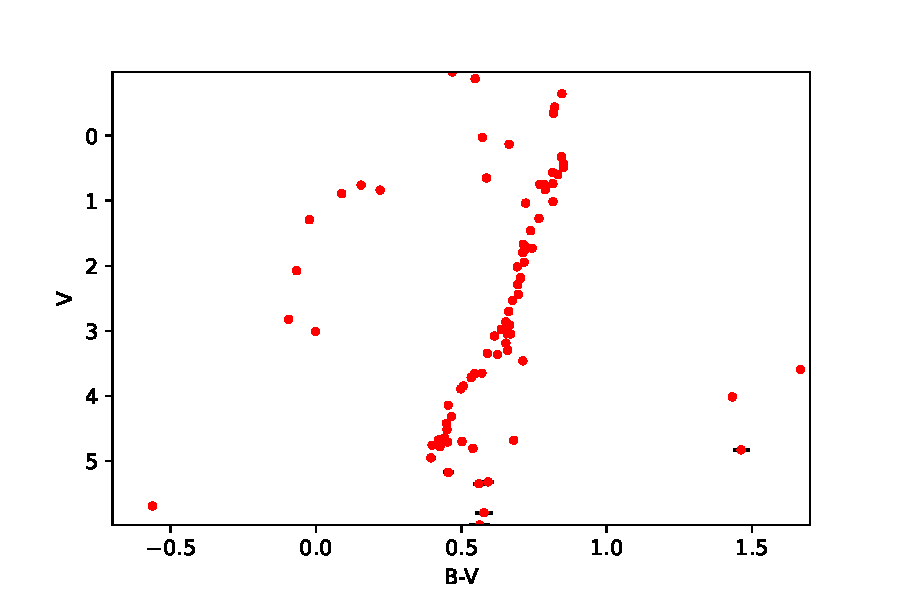
\includegraphics[width=0.45\paperwidth]{B-V}
	\caption{Graph of the 80 stars in M13 V magnitude vs their (B-V) magnitude (H-R diagram). The error bars represent the error in recording the magnitude }
	\label{fig:b-v}
\end{figure}

A H-R diagram of M13 from the data in Table \ref{tab:table} is shown in Figure \ref{fig:b-v}. The V magnitude is shown on the y-axis and the B magnitude minus the V magnitude (B-V) is shown on the x-axis. This has produced a graph of absolute magnitudes of stars in M13 with a defined line of stars that represent the main sequence and the evolution onto the RGB. Looking at Figure \ref{fig:b-v} the main sequence turn off looks to be roughly around 4 in V and 0.5 in B-V. Using the graphs of isochrone models in \citet[pg.73]{labhandbook} a rough primary estimate for the age of M13 is 16 Gyr assuming that [Fe/H] in the cluster is -1.27. 
\begin{figure}[H]
	\centering
	\begin{subfigure}[t]{0.35\paperwidth}
	\centering
	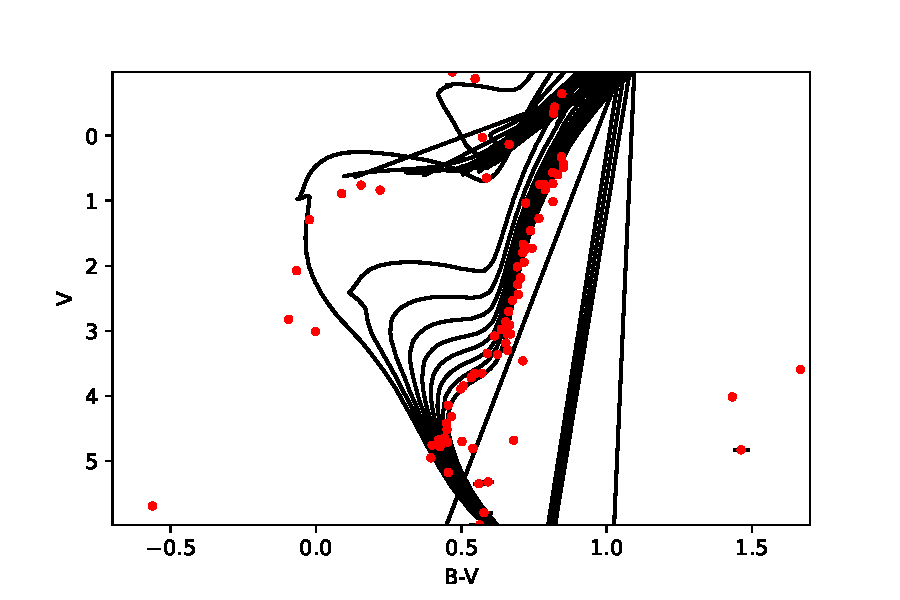
\includegraphics[width=\textwidth]{isofitwhole}
	\caption{Several Isochrone fits}
	\label{fig:isowhole}
	\end{subfigure}
	\begin{subfigure}[t]{0.35\paperwidth}
	\centering
	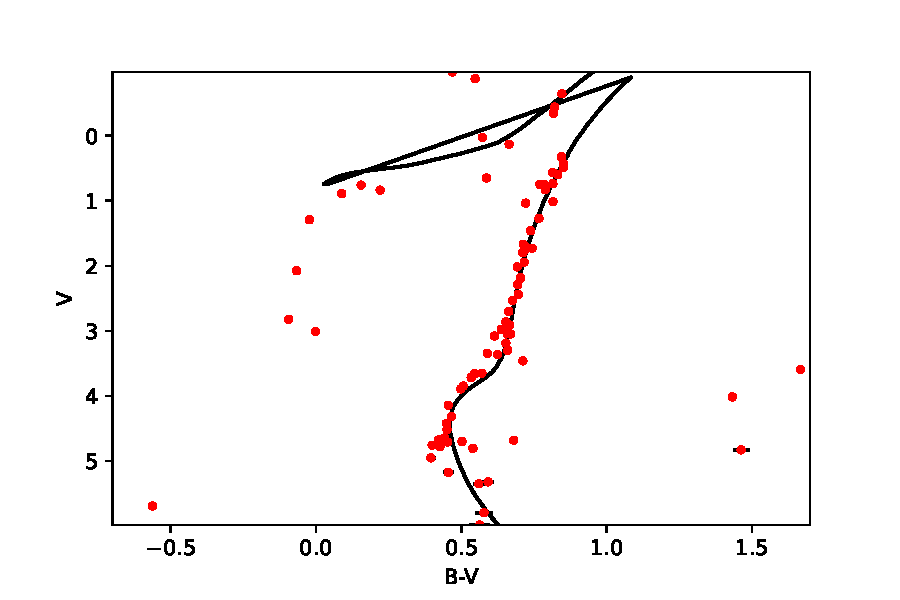
\includegraphics[width=\textwidth]{isofit17.pdf}
	\caption{Isochrone fit that most closely matches}
	\label{fig:iso}
	\end{subfigure}
	\caption{H-R diagram of the stars in M13. Figure \ref{fig:isowhole} shows half of the isochrone model fits by \citet{Rey_2001}. Figure \ref{fig:iso} has the isochrone that most closely matches the main sequence turn off and has an age of 18 Gyr}
	\label{fig:isochronefigures}
\end{figure}

A more accurate way of determining the best isochrone model fit is by directly plotting them onto the H-R diagram and determining which model fits the best. To do this data of several isochrone fits using a [Fe/H] = -1.33 from \citet{Rey_2001} were imported into python and can be seen in Figure \ref{fig:isowhole}. The isochrone model that best fits the data is shown in Figure \ref{fig:iso} and has an age of 18 Gyr. It is hard to determine an error value for the age as it was not worked out by direct calculation but instead by selecting a model that looks closest to the main sequence turn off. However during the determination of the best isochrone fit there were several models that could be potentially be the best fit but were not chosen so an uncertainty in the age was decided as the range of these values resulting in the age of M13 being $18^{+0}_{-4}$ Gyr.

There are also some outlier stars in the data where they do not fit on the main sequence, this could be due to: errors/mistakes in using the aperture photometry tool, selecting stars that are not actually in the cluster and not taking the magnitude of the same star in both filters due to large quantity of stars and their difficulty in distinguishing them. To ensure that only the stars that are in M13 are plotted the position of each star recorded should be cross referenced with a database of the known positions of M13 stars so that any outliers can be removed.

When recording the values for the magnitudes stars would be selected by their size and separation from other objects to allow for the easiest and most accurate aperture photometry result. This meant that most stars selected were focused around the outer edge of the cluster and were more luminous as shown in Figure \ref{fig:position}. This could introduce a distortion of the stellar contents in M13, favouring lower magnitude stars (more negative), potentially creating an inaccurate main sequence turn off. Therefore to test if this plays a role in the determination of the age of the cluster a plot of all the stars in M13 is shown in Figure \ref{fig:reydata} with data from \citet{Rey_2001}.
\begin{figure}[h]
	\centering
	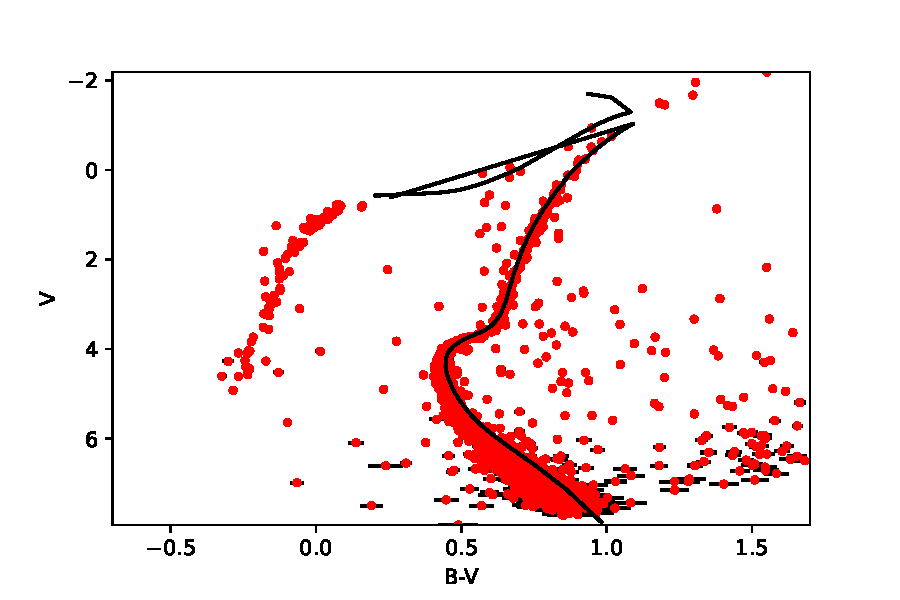
\includegraphics[width=0.45\paperwidth]{rey}
	\caption{H-R diagram using data from \citet{Rey_2001} The isochrone that most closely fit the main sequence turn off has an age of 16 Gyr}
	\label{fig:reydata}
\end{figure}

The best isochrone model fit with this data produced an age of 16 Gyr which is not the same result as the plot with 80 stars. This shows that most of the stars in the cluster need to be recorded to produce the most accurate result for the age, as in this experiment 80 stars was not enough. In both Figure \ref{fig:reydata} and \ref{fig:iso} the error bars in the magnitudes increased with larger magnitudes (more positive) which is likely due to the stars lower luminosities and the greater impact of overlapping stars on the calculation of its magnitude in Gaia.

According to \citet{VandenBerg_2013} M13 has an age of ($12.00 \pm 0.38$) Gyr which is in agreement with \citet{Grundahl_1998} value of ($12.00 \pm 1.50$) Gyr. Both of these values disagree with the value for the age obtained in this experiment. In \citet{VandenBerg_2013}, \citet{Grundahl_1998} and \citet{Rey_2001} the average metallicity of M13 was taken as [Fe/H] = -1.6 which is different from the value used in this experiment. This means that the isochrone models used were not accurate for the stellar composition of M13 and cannot give a result for its age. The most resent study on the stellar population in M13 suggests that the metallicity is [Fe/H] $=(-1.58 \pm 0.09)$ \citep{deras}. Therefore in the future isochrone models used to analyse M13 need to take this into account. The distance to M13 found by \citet{deras} and \citet{buckley} was 7.1 kpc which is different to the value used in this experiment of 6.8 kpc \citep{Paust_2010}. Do note that in the \citet{buckley} study they use a [Fe/H] = -1.4 so the validity of their results could be questioned. This difference in distance would cause incorrect values for the absolute magnitude of stars in M13 and also result in inaccurate age estimates as the isochrone models selected would not match the actual properties of the cluster. Therefore the results obtained in this experiment are inaccurate and cannot be used as definitive values of the properties of M13.

In the future to reduce error the isochrone models should be fitted to the data in a more accurate way instead of the human observation technique used in this report. Using a least square fit of the data with the isochrone models would select the closet match and eliminated the human uncertainty. Furthermore This would introduce a measurable uncertainty in the age which would allow for further analysis of the result. 

\section{Conclusion}
In this report Images of M13 taken by CFHT in the B and V filters were used to analyse the stellar evolution in the cluster. To do this aperture photometry was performed on 80 stars in the cluster and plotted onto a H-R diagram. Using isochrone models the main sequence turn off was determined and the age of the cluster was found to be $18^{+0}_{-4}$ Gyr. This value is in disagreement with \citet{VandenBerg_2013} and \citet{Grundahl_1998} who found the age of M13 to be 12 Gyr. In this experiment the metallicity of M13 was taken as [Fe/H] = -1.33 which is different from the value used by \citet{VandenBerg_2013} and \citet{Grundahl_1998}. A recent Study of M13 found that the metallicity is [Fe/H] = $=(-1.58 \pm 0.09)$ \citep{deras} so this experiment has used inaccurate isochrone models to find the age of the cluster. Further analysis of the age determination method found that the isochrone fitting technique is inaccurate so future isochrone fittings should use a least square fitting technique or other computer determined fits. Therefore this experiment has not produced an accurate result for the age of M13 but has found methods to improve the accuracy of analysis in future experiments.


\bibliographystyle{agsm}
\bibliography{cluster.bib}
\pagebreak
\section*{Appendix}
\begin{figure}[H]
\centering
	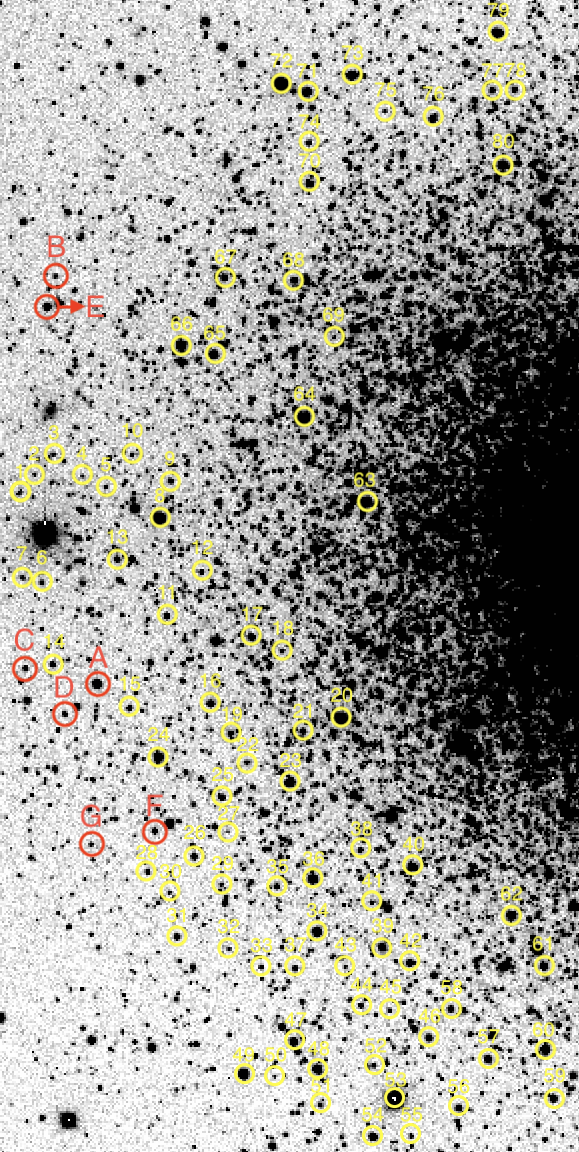
\includegraphics[width=0.55\textwidth]{positions}
	\caption*{Larger version of Figure \ref{fig:position}}
\end{figure}
\end{document}





